%-------------------------------------------------------------------------------
% File: main.tex
%	COVID-19 Behind the Numbers project documentation.
%
%	Compile using:
%	    $ pdflatex main.tex
%	    $ biber main
%
% Author: Rambod Rahmani <rambodrahmani@autistici.org>
%	  Created on 07/01/2021
%-------------------------------------------------------------------------------
\documentclass[11pt,a4paper]{article}

\usepackage[a4paper, portrait, margin=1.1in]{geometry}
\usepackage[dvipsnames]{xcolor}
\usepackage[linktoc=none]{hyperref}
\hypersetup{
	colorlinks=true,
	linkcolor=blue,
	filecolor=magenta,      
	urlcolor=blue,
}
\usepackage{listings}
\usepackage{float}
\usepackage{graphicx}
\usepackage[justification=centering]{caption}
\usepackage{wrapfig}
\usepackage{amsmath}
\usepackage{bold-extra}

% time series countries colors
\definecolor{ts_belgium}{rgb}{0.11, 0.46, 0.70}
\definecolor{ts_armenia}{rgb}{0.99, 0.49, 0.5}
\definecolor{ts_austria}{rgb}{0.16, 0.62, 0.16}
\definecolor{ts_bulgaria}{rgb}{0.83, 0.14, 0.15}
\definecolor{ts_france}{rgb}{0.57, 0.40, 0.73}
\definecolor{ts_unitedstates}{rgb}{0.54, 0.33, 0.29}
\definecolor{ts_spain}{rgb}{0.88, 0.46, 0.75}
\definecolor{ts_germany}{rgb}{0.49, 0.49, 0.49}
\definecolor{ts_italy}{rgb}{0.73, 0.73, 0.12}
\definecolor{ts_brazil}{rgb}{0.0, 0.100, 0.84}

% bibliography references
\usepackage[backend=biber,style=numeric,sorting=none]{biblatex}
\addbibresource{main.bib}
\nocite{*}

%-------------------------------------------------------------------------------
% Document
%-------------------------------------------------------------------------------
\begin{document}

%-------------------------------------------------------------------------------
% Title
%-------------------------------------------------------------------------------
\begin{center}
	\huge{\bfseries{COVID-19: Behind The Numbers}}\\
	\vspace{1.0cm}
	\large{Data Mining and Machine Learning Project}\\
	\vspace{0.2cm}
	\large{Prof. Marcelloni Francesco}\\
	\vspace{0.2cm}
	\large{Prof. Ducange Pietro}\\
	\vspace{1.0cm}
	\large\textit{Rambod Rahmani}\\
	\vspace{0.2cm}
	\scriptsize{Master's Degree in Artificial Intelligence and
	Data Engineering}\\
	\vspace{1.0cm}
	\normalsize{\today}
\end{center}

%-------------------------------------------------------------------------------
% Table of contents
%-------------------------------------------------------------------------------
\vspace{2.0cm}
\tableofcontents

%-------------------------------------------------------------------------------
% Section: Introduction
%-------------------------------------------------------------------------------
\newpage
\section{Introduction}
\textbf{Decemebr 31, 2019}: \textit{China, Wuhan Municipal Health Commission
reported a cluster of cases of pneumonia in Wuhan, Hubei Province.}\\
\\
\textbf{January 1, 2020}: \textit{World Health Organization (WHO) had set up the
Incident Management Support Team across the three levels of the organization.}\\
\\
\textbf{January 5, 2020}: \textit{WHO published the first Disease Outbreak News
on the new virus. This was a flagship technical publication to the scientific
community.}\\
\\
\textbf{January 12, 2020}: \textit{China publicly shared the genetic sequence of
COVID-19.}\\
\\
At the beginning of 2020, a new virus started spreading around in the capital of
Central China's Hubei province: the city we all came to know as Wuhan. As it
turned out, this was the start of a world-changing event with overwhelming
extent: Coronavirus Disease 2019 (COVID-19). After the first and the second
waves of the virus have passed over the entire world, while the number of deaths
by COVID-19 infections is decreasing as a result of the vaccination campaigns,
the aim of this work is to address the following questions:
\begin{itemize}
	\item \textbf{Which countries have been affected the most by COVID-19?}
	\item \textbf{Is it possible to build personalized predictive models for
		symptomatic COVID-19 patients based on health preconditions?}
\end{itemize}
In order to fully answer these questions, first of all a reliable and big enough
dataset is needed. Second, data mining and machine learning techniques can be
applied in order to obtain statistically significant results that could help
address the proposed questions. In the following pages the development of the
project and the resulting Python software are presented. The software
architecture is presented in the very last section in order to focus primarily
on the dataset retrieval and preprocessing, and on the analysis techniques and
results.\\
\\
All the files related to this work are available in this GitHub repository:
\url{https://github.com/rambodrahmani/covid19-behind-the-numbers}

%-------------------------------------------------------------------------------
% Section: Dataset
%-------------------------------------------------------------------------------
\newpage
\section{Dataset}
Two different datasets were used:
\begin{itemize}
    \item the data on confirmed cases and confirmed deaths is updated daily and
    is published by the \textbf{Johns Hopkins University}; this is the best
    available dataset on the pandemic at global level;
    \item as far as it concerns medical preconditions of COVID-19 patients,
    the most detailed dataset I was able to retrieve is the one provided by
    \textbf{The Federal government of Mexico}.
\end{itemize}
The content of the datasets, the features of interest used in what follows and
the preprocessing procedures applied on each of them are detailed in the
following subsections.
\subsection{COVID-19 Daily Data}
The Johns Hopkins University Center for Systems Science and Engineering
(JHU CSSE)\footnote{\url{https://coronavirus.jhu.edu/map.html}} provides the
best available global dataset on the COVID-19 pandemic. Multiple sources were
used in the data set, since January 21, 2020:
\begin{itemize}
    \item World Health Organization (WHO);
    \item European Centre for Disease Prevention and Control (ECDC);
    \item US Centers for Disease Control and Prevention (UCDC);
    \item Los Angeles Times;
    \item The Mercury News.
\end{itemize}
The JHU CSSE data is provided as a collection of daily \texttt{.csv} files which
need to be merged to obtain the dataset with all the daily data for all the
countries. Luckily, the \textbf{Our World in Data} organization --- a
collaborative effort between researchers at the University of Oxford, focused on
"research and data to make progress against the world's largest problems" ---
provides the JHU CSSE data already
merged\footnote{\url{https://ourworldindata.org/coronavirus-data}} and updated
to the latest second as a single \texttt{.csv} file. The choice was made to use
this \texttt{.csv} file as dataset.\\
The dataset file is named \texttt{owid-covid-data.csv} with a size of $26.2$
MiB.\\
\\
This dataset was used for the first part of the work: finding the characteristic
curves of each country and grouping together countries with comparable behavior
by means of time series clustering algorithms. This will provide us a truthful
overview of the countries most affected by COVID-19 and the ones that put in 
place appropriate policies to handle the pandemic widespread.
\subsubsection{Preprocessing}
This dataset contains worldwide, per-country, daily data for COVID-19 for a
total of 59 columns and $103349$ entries. Among others, we are interested mainly
in the following features:
\begin{itemize}
    \item total confirmed cases;
    \item new confirmed cases;
    \item total deaths;
    \item new deaths;
    \item total confirmed cases per one million population;
    \item new confirmed cases per one million population;
    \item total deaths per one million population;
    \item new deaths per one million population.
\end{itemize}
The main considerations to be made about this dataset as far as it concerns data
preprocessing are:
\begin{itemize}
    \item it contains redundant data, e.g. values aggregated by continent (Asia,
    Africa, Europe, America, North America etc\dots);
    \item some of the daily data values are missing (specially for the very
    initial months of the pandemic, i.e. from 2020-01-01 to 2020-03-01);
    \item some of the daily data values are negative;
\end{itemize}
as a result, the following preprocessing procedures were applied
\begin{itemize}
    \item data aggregated by continents was removed;
    \item missing daily data values for countries were replaced\footnote{The
    \texttt{scikit-learn SimpleImputer} was used to this end.} with the constant
    value $0$; this seems the most reasonable choice since these missing values
    refer to the very beginning of the pandemic; using either the mean or the
    mode results a distorted dataset;
    \item negative values were replaced using the moving average\footnote{The
    \texttt{pandas DataFrame.rolling} method was used to this end.} with a
    moving window of size $15$ to approximate the negative values as the average
    of the $7$ previous and successive values.
\end{itemize}
Taking into account also the fact that the daily data will mostly be used
resampled with weekly frequency and that by visual inspection it appears that
negative values are close to zero, there is no need to further preprocess this
dataset.
\subsection{COVID-19 Medical Preconditions Data}
The second part of this work focused on frequent pattern analysis in order to be
able to find interesting patterns as far as it concerns COVID-19 patients who
had prior medical preconditions. Finding such patterns is a crucial task that
might allow to best allocate very limited medical resources. The rapid global
spread of the virus SARS-CoV-2 has provoked a spike in demand for hospital care.
Hospital systems across the world have been over-extended, including the one
case we are most familiar with, Northern Italy.
As a result, decisions on how to best allocate very limited medical resources
have come to the forefront: who to test, who to admit into hospitals, who to
treat in an Intensive Care Unit (ICU), who to support with a ventilator.\\
\\
The dataset required for such type of analysis was not easy to find: usually
COVID-19 datasets only contain daily values (numbers) of confirmed cases and
deaths. They rarely come equipped with the medical preconditions of the
patients. Luckily, the Federal government of Mexico\cite{mexico} provided such a
dataset. It is splitted in three main files:
\begin{itemize}
    \item \texttt{210206COVID19MEXICO.csv}: the main file containing, among
    others,
    \begin{itemize}
        \item patients sex, age, admission date, COVID-19 test result;
        \item if the patient required hospitalization, intubation or Intensive
        care unit (ICU);
        \item if the patient was affected by Pneumonia, Diabetes, Asthma,
        Hypertension, Cardiovascular disease (CVD), etc\dots;
        \item death date (only for those patients who actually died).
    \end{itemize}
    \item \texttt{201128\_Catalogos.xlsx}, \texttt{201128\_Descriptores.xlsx}:
    contain additional clarifications regarding each feature present in the main
    dataset file.
\end{itemize}
This dataset is perfect for the objective of the analysis we are interested in
--- develop personalized models that predict the following events:
\begin{enumerate}
    \item hospitalization;
    \item need for ICU;
    \item need for a ventilator;
    \item mortality.
\end{enumerate}
\subsubsection{Preprocessing}
The preprocessing required by this second dataset is completely different from
the one required  by the first one. This is because the type of data is
completely different. While the first dataset is primarily a sequence of
numerical records, here we deal with categorical attributes. The main
considerations to be made include:
\begin{itemize}
    \item the dataset is split into $3$ files: one with the main content, the
    remaining two files contain headers details;
    \item Spanish is the de facto national language spoken by the vast majority
    of Mexicans, all files are in Spanish;
    \item the dataset has a size of about $990$ MiB, with a total of 40 columns
    and more than 6.000.000 entries.
\end{itemize}
The preprocessing stage included merging the 3 files into a single \texttt{.csv}
file, in English, containing therefore patients details, medical preconditions,
required medical care and if they survived SARS-CoV-2 or not.

%-------------------------------------------------------------------------------
% Section: Analysis
%-------------------------------------------------------------------------------
\newpage
\section{Analysis}
As said in the introductory section, the analysis was carried out using data
mining and machine learning techniques in order to answer the proposed
questions. As we move on to build our models, in this very particular case,
working with data from a pandemic such the COVID-19, we should do that by
\textbf{taking a very critical look at models}. Keep in mind the aphorism "All
models are wrong", often expanded as "All models are wrong, but some are
useful". The modeller's paradox is even more true when crisis erupts:
unfortunately, in such situations, data are lacking or of poor quality. What is
worse is that models do not simulate the behaviours of citizens to stop seeking
medical assistance in the case of a pandemic (because of fear), models do not
capture the effects of sustained lock down as far as it concerns mental health
and general social well being. Models can not simulate the social and economical
consequences of business failures and economic depressions, nor do models
simulate the effects of increase of violence and policing on cultural norms or
attitudes towards democracy. And also importantly, is that models do not
translate well necessarily across different cultural and political boundaries.
\subsection{Which countries have been affected the most by COVID-19?}
To answer the very first question, we need to understand what is hidden behind
the official numbers and charts of confirmed COVID-19 active cases and deaths.
We are not doing anything clever at all, just plotting the data and trying to
learn from it.\\
\\
We are so used to watching COVID-19 numbers and charts nowadays and sometimes we
think we might even understand how the pandemic is evolving as days goes by. For
example, it is very common to consider the following plot:
\begin{figure}[H]
    \begin{center}
        \hspace*{-0.2cm}
        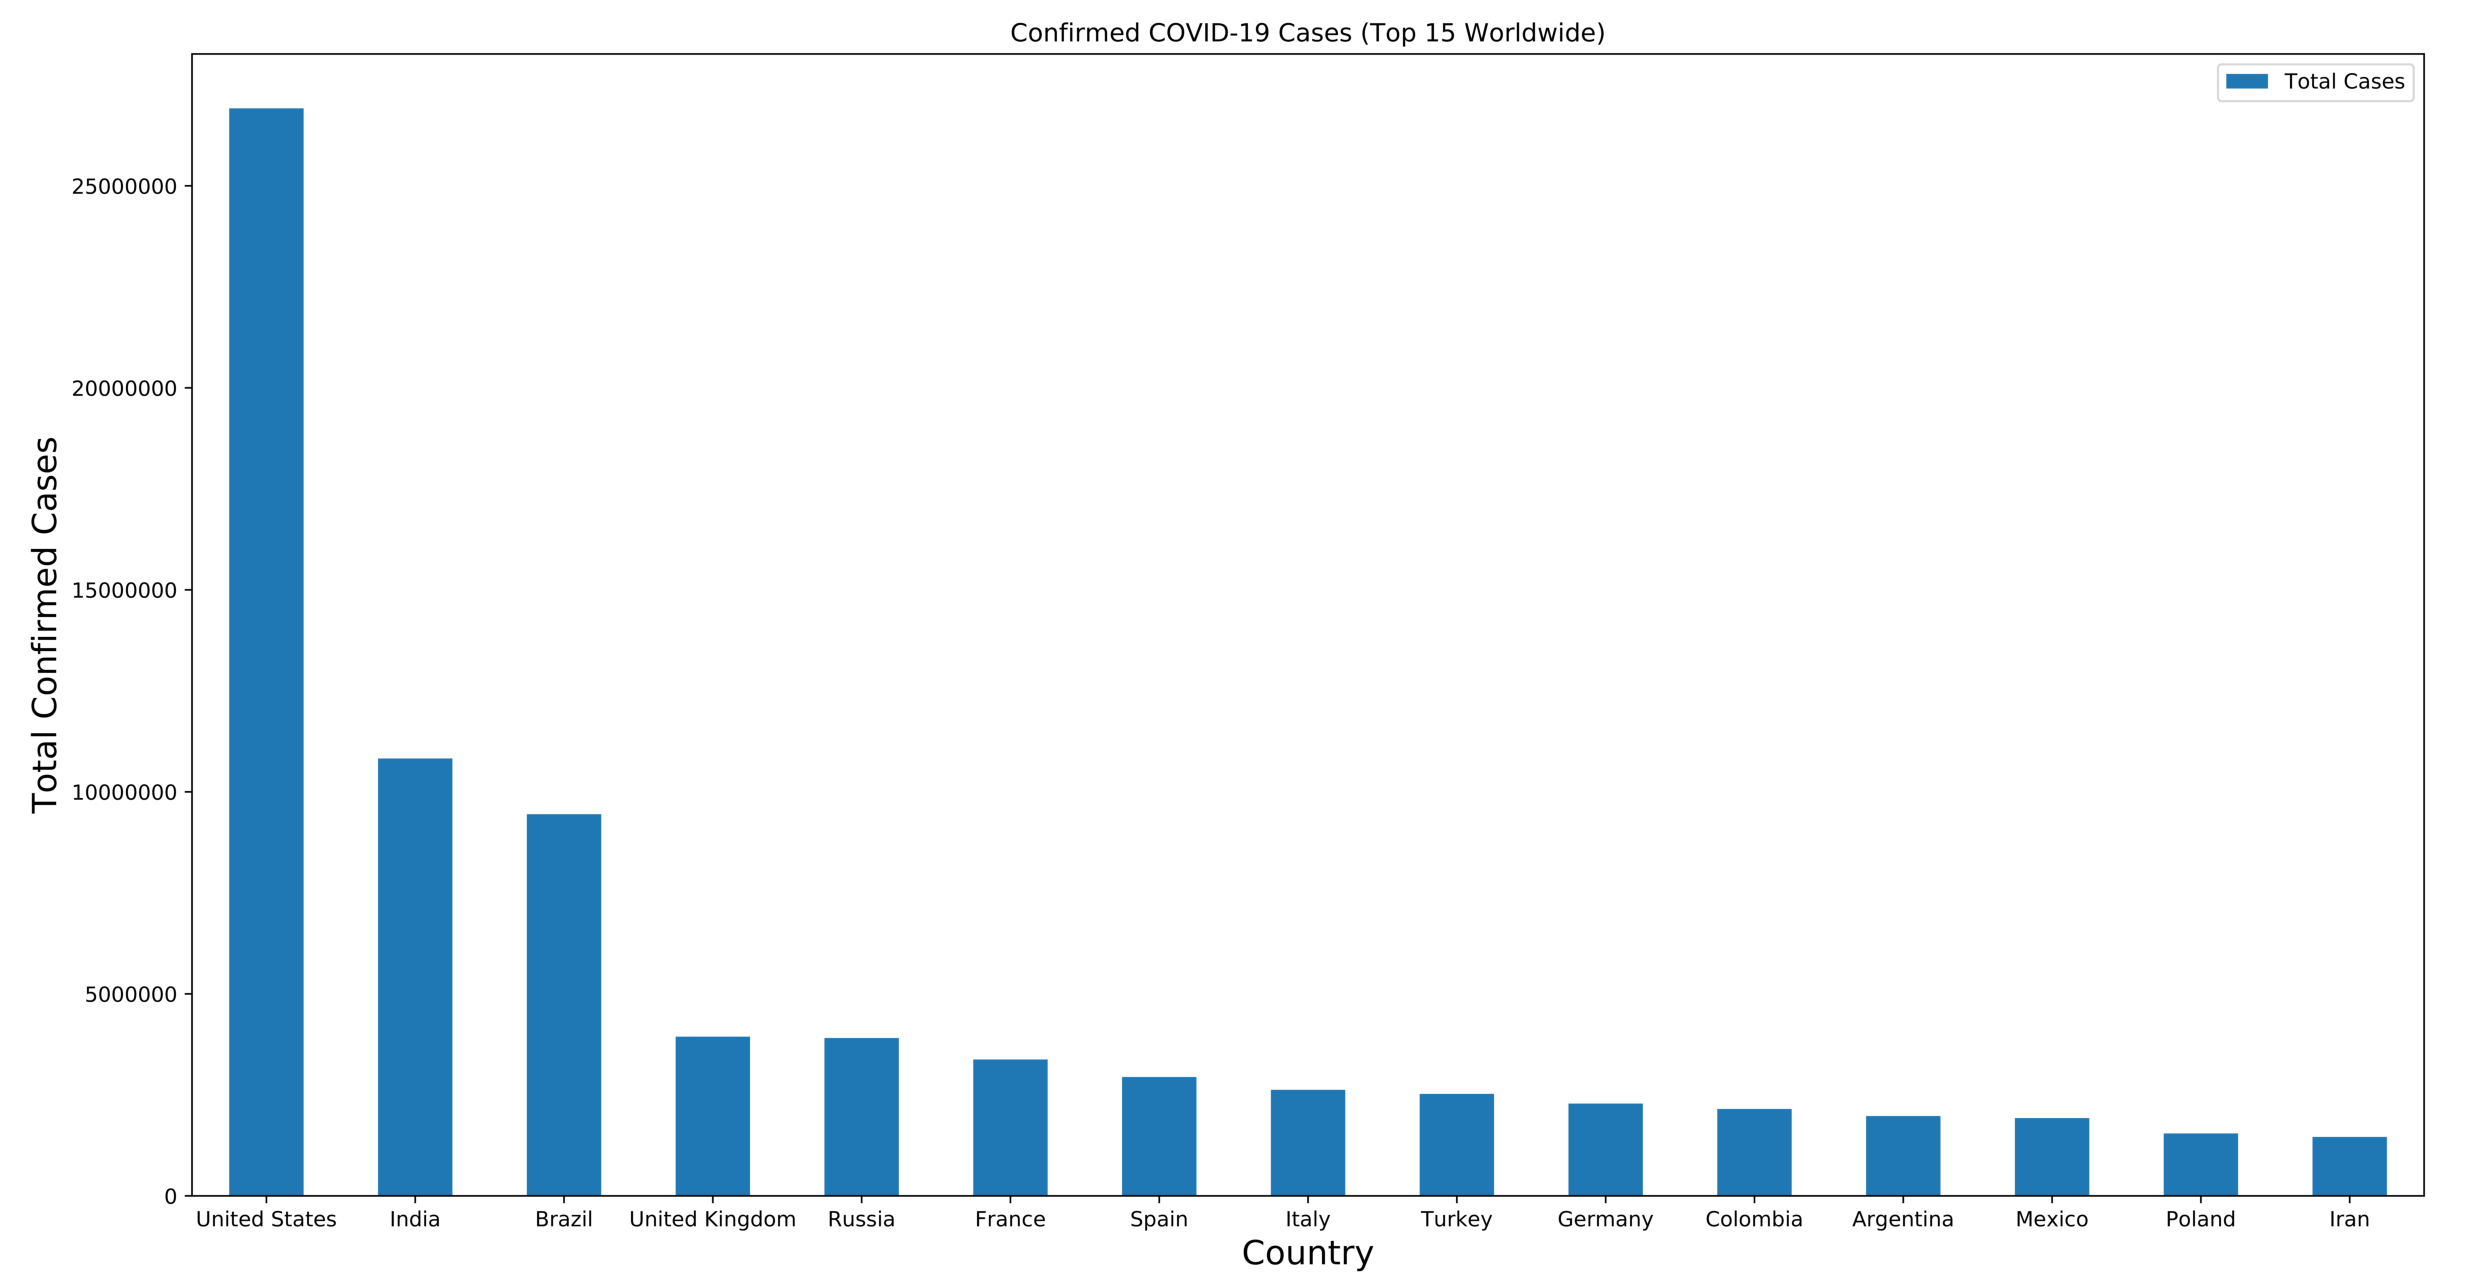
\includegraphics[scale=0.32]{img/total-cases.pdf}
    \end{center}
    \vspace{-0.3cm}
    \caption{Top 15 Countries Confirmed COVID-19 Cases}
\end{figure}
\noindent
Is this really the right choice? Does this ranking tells us anything meaningful
about the current undergoing pandemic situation? From what we can observe in
figure 1, clearly United States has higher confirmed COVID-19 cases than
countries such as Spain or Italy. Taking into account that the US is a much
bigger country, we can agree that this results do not imply that the US is more
affected than Spain, Italy or Germany. We can therefore think of a fairer
comparison independent of the country size: the number of infections needs to be
normalized to the population of each country. This provides a more coherent view
of the countries most affected by COVID-19:
\begin{figure}[H]
    \begin{center}
        \hspace*{-0.2cm}
        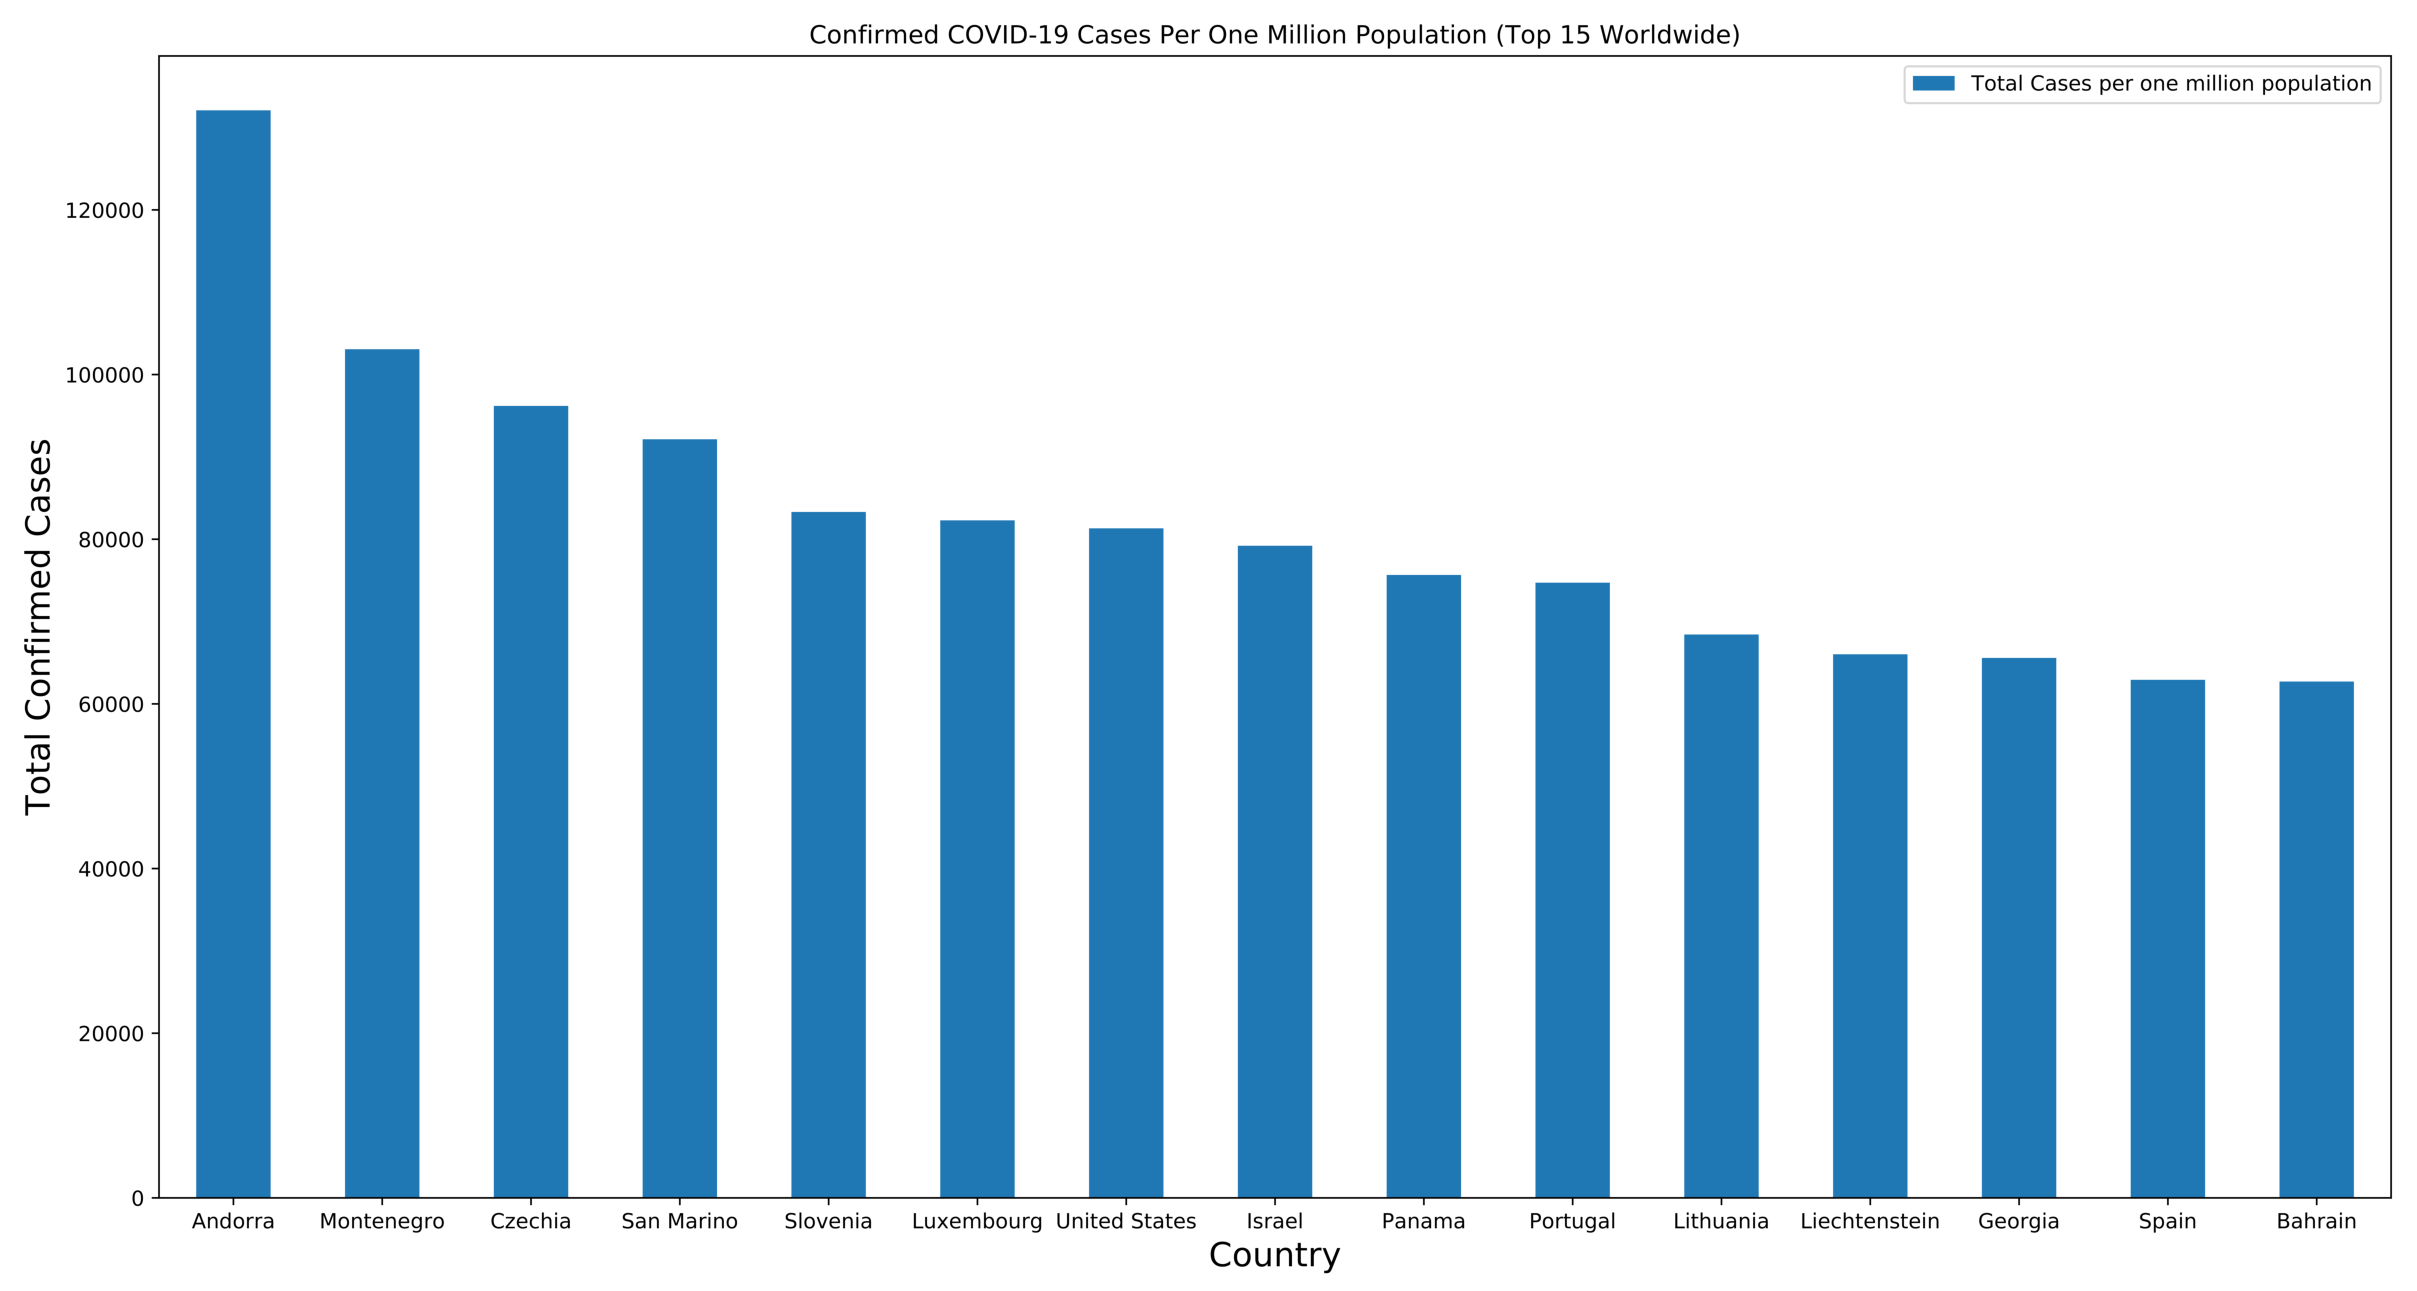
\includegraphics[scale=0.32]{img/total-cases-per-million.pdf}
    \end{center}
    \vspace{-0.3cm}
    \caption{Top 15 Countries Confirmed COVID-19 Cases Per One Million Population}
\end{figure}
\noindent
However it is not yet good enough: countries have different testing policies and
a more intensive COVID-19 testing rate gives more confirmed cases while no
testing at all would imply zero cases. We can all agree upon the fact that zero
cases with no testing at all does not really mean that a given country is not
affected by the pandemic. We therefore need a quantity unrelated to the rate of
testing.\\
This quantity is the number of deaths: this value is unbiased by the testing
rate. We will use the normalized number of daily deaths for comparing
countries.\\
\\
Before moving on, it is important to clarify that when we deal with COVID-19
deaths we refer to number of people who died in the COVID-19 time period
(starting from January 2020 till today). It is important to point out that
on the death certificate of these individuals there might be no reference at
all to the COVID-19 pandemic. This is because, as a result of different
policies in different countries worldwide, it is hard to obtain reliable
datasets with daily deaths that differentiate between those labeled COVID-19
and those completely related to other causes. Additionally, sometimes there is
no certainty about whether COVID-19 did or did not play a role in the death of
an individual.\\
\\
While the previous results were obtained using the original COVID-19 historical
dataset\cite{ourworldindata}, \textbf{this time some preprocessing and
resampling is needed}:
\begin{itemize}
    \item the daily values for some of the dates in the original dataset are missing:
    \begin{itemize}
        \item countries with too many missing values (more than $150$ days) were
        removed since no interpolation technique can really be effective in such
        cases;
        \item where few missing values were present, these were replaced using
        the constant value $0$;
    \end{itemize}
    \item plotting the data with daily granularity results in a time series plot
    which is not smooth and hard to read; the data was therefore resampled with
    weekly granularity;
\end{itemize}
To impute the missing values, i.e., to infer them from the known part of the
data, an univariate imputation algorithm was used: imputes values in the
i-th feature dimension using only non-missing values in that feature dimension.
To this end, the \texttt{SimpleImputer} class from the \texttt{scikit-learn}
Python package and the \texttt{rolling} method from the
\texttt{pandas.DataFrame} package were used.\\
\\
This is the resulting time series plot for some of the countries:
\begin{figure}[H]
    \begin{center}
        \hspace*{-0.3cm}
        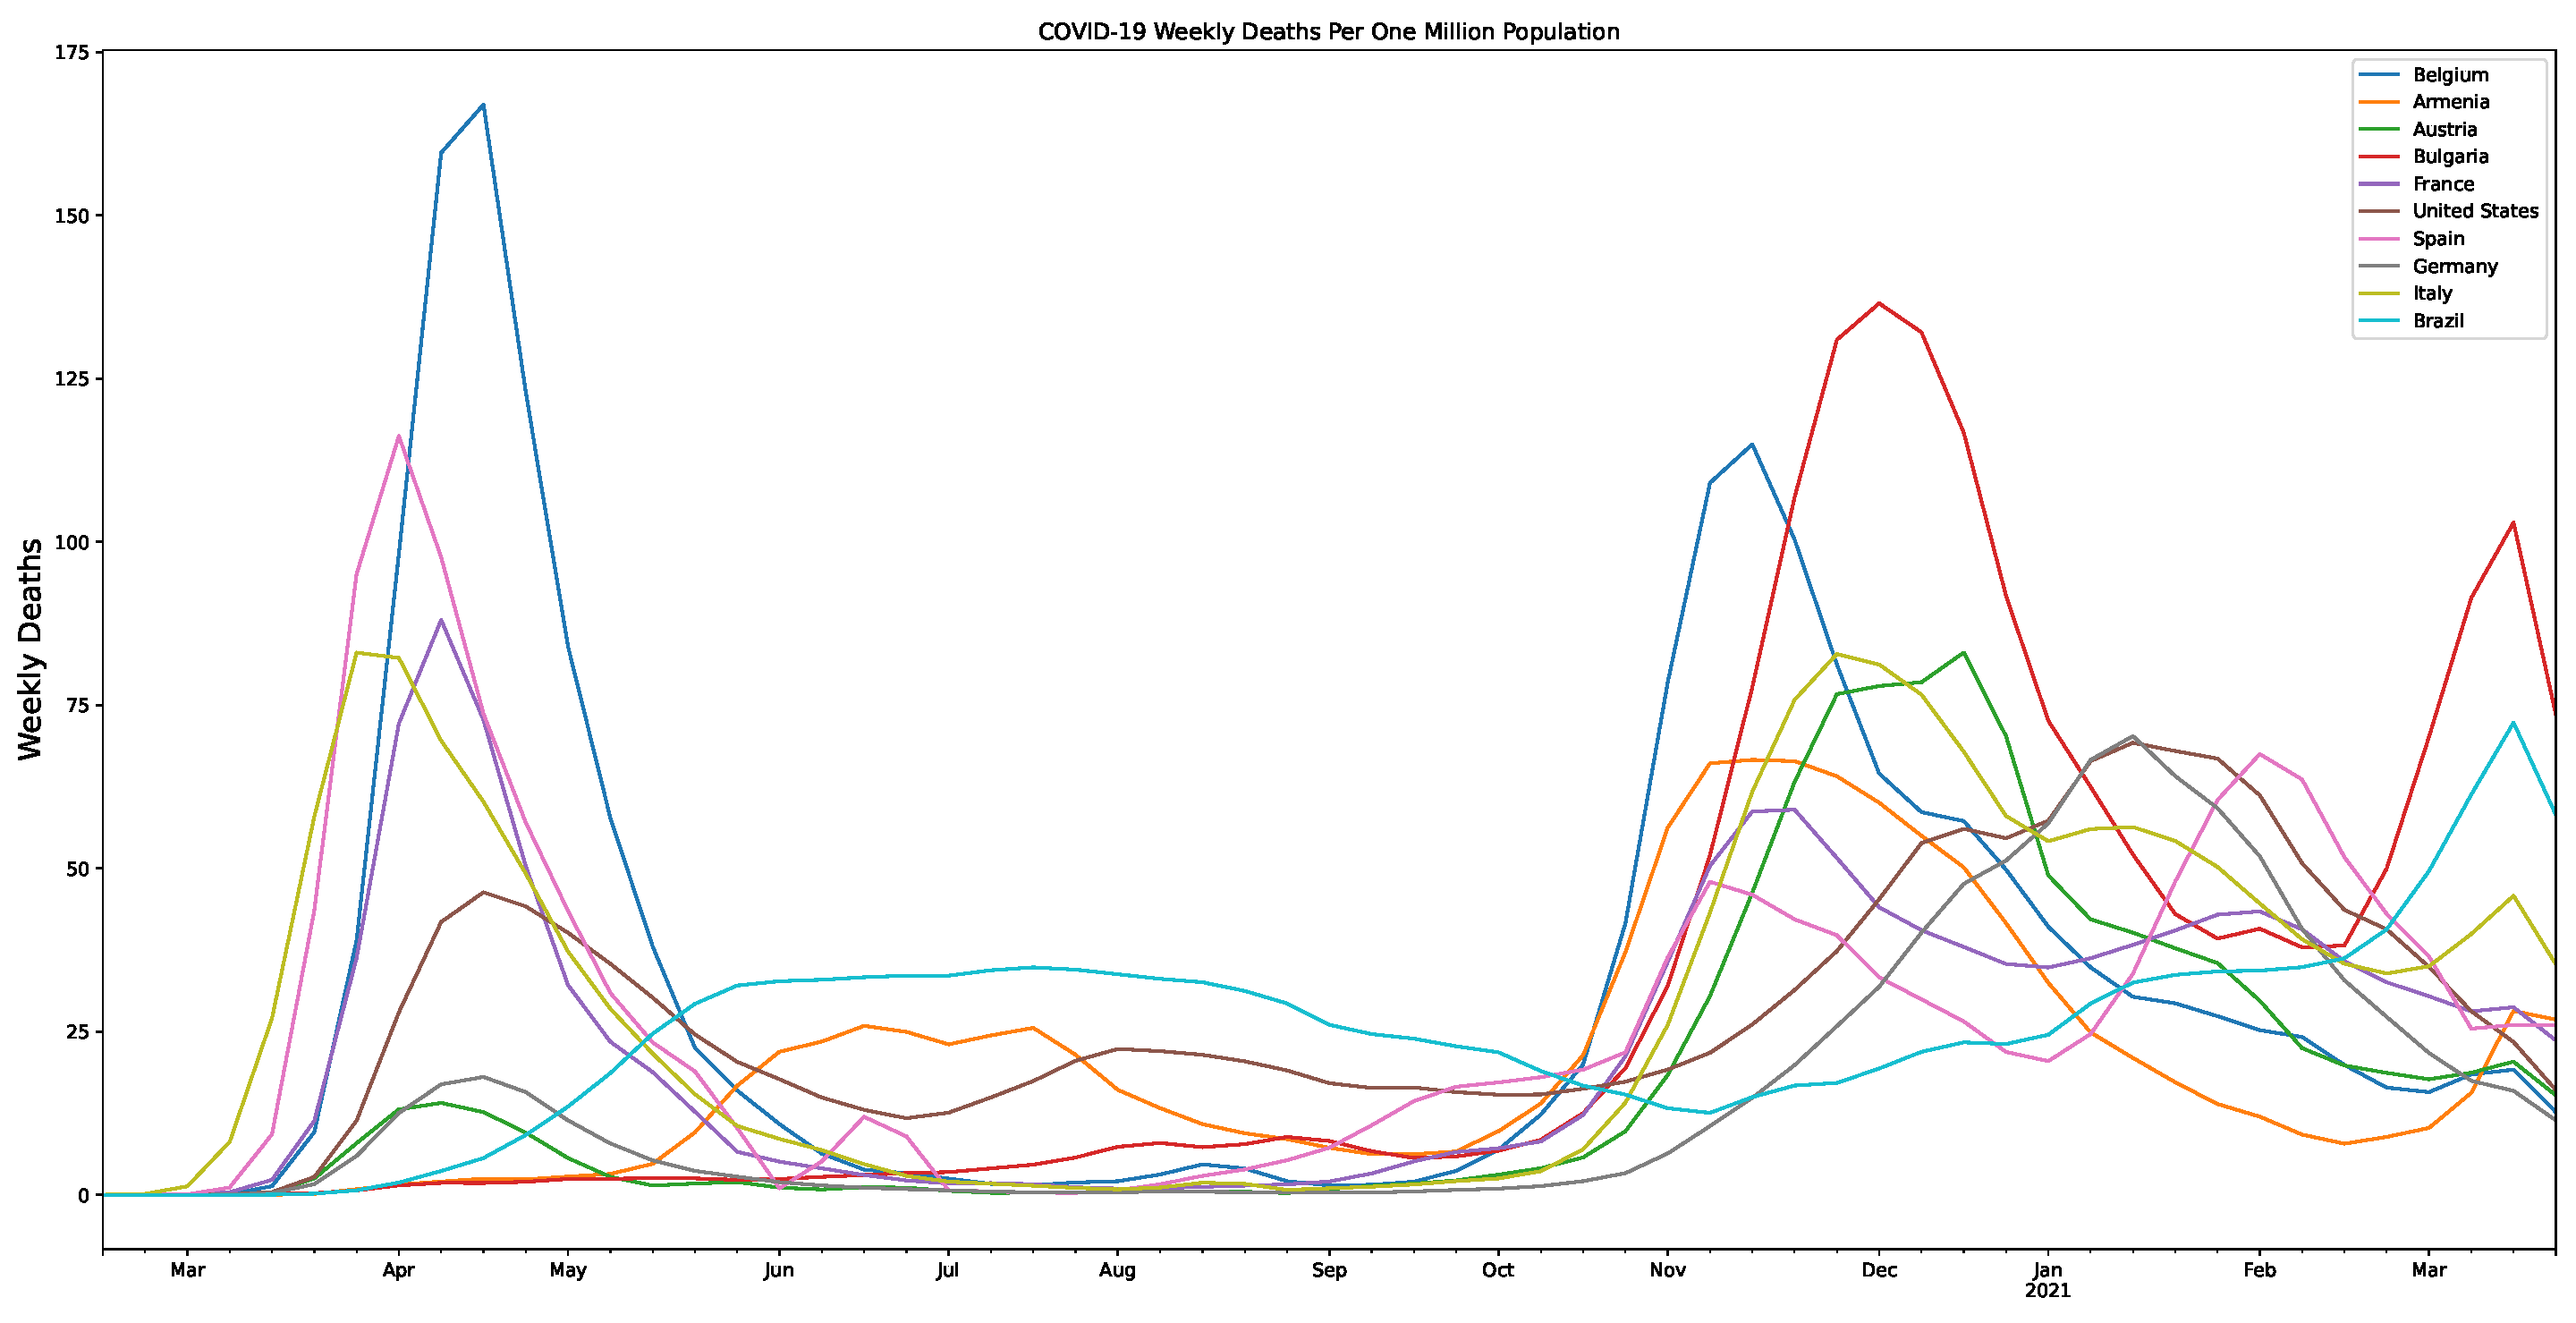
\includegraphics[scale=0.325]{img/weekly-deaths-per-million.pdf}
    \end{center}
    \vspace{-0.3cm}
    \caption{COVID-19 Weekly Deaths Per One Million Population}
\end{figure}
\noindent
Daily deaths count appears to be a fair measure to compare how hard different
countries have been hit by the virus. In addition, observing the plot one can
immediately point out that
\begin{itemize}
    \item some countries suffered more the first wave, some others the second
    and some both;
    \item countries such as {\color{ts_italy}Italy} and
    {\color{ts_belgium}Belgium} were devastated by the first wave and reacted
    by completely shutting down social life; yet they are not doing better with
    the second wave;
    \item countries such as {\color{ts_austria}Austria} and
    {\color{ts_germany}Germany} have not been hit hard by the first COVID-19
    wave; these states reacted fast and slowed down social life right at the
    beginning; as a result, the number of deaths went back to almost zero; yet
    they are suffering from the second wave;
    \item countries such as {\color{ts_unitedstates}United States} and
    {\color{cyan}Brazil} have a daily death toll with an almost constant
    trend.
\end{itemize}
If we extend the same reasoning to all the countries, figure 4 shows the weekly
deaths per one million population for 200 countries, from Afghanistan to
Zimbabwe. It is humanly impossible to extract any useful information from such a
plot. However, in this mess, how many different characteristic curves can we
find?
\begin{figure}[H]
    \begin{center}
        \hspace*{-0.3cm}
        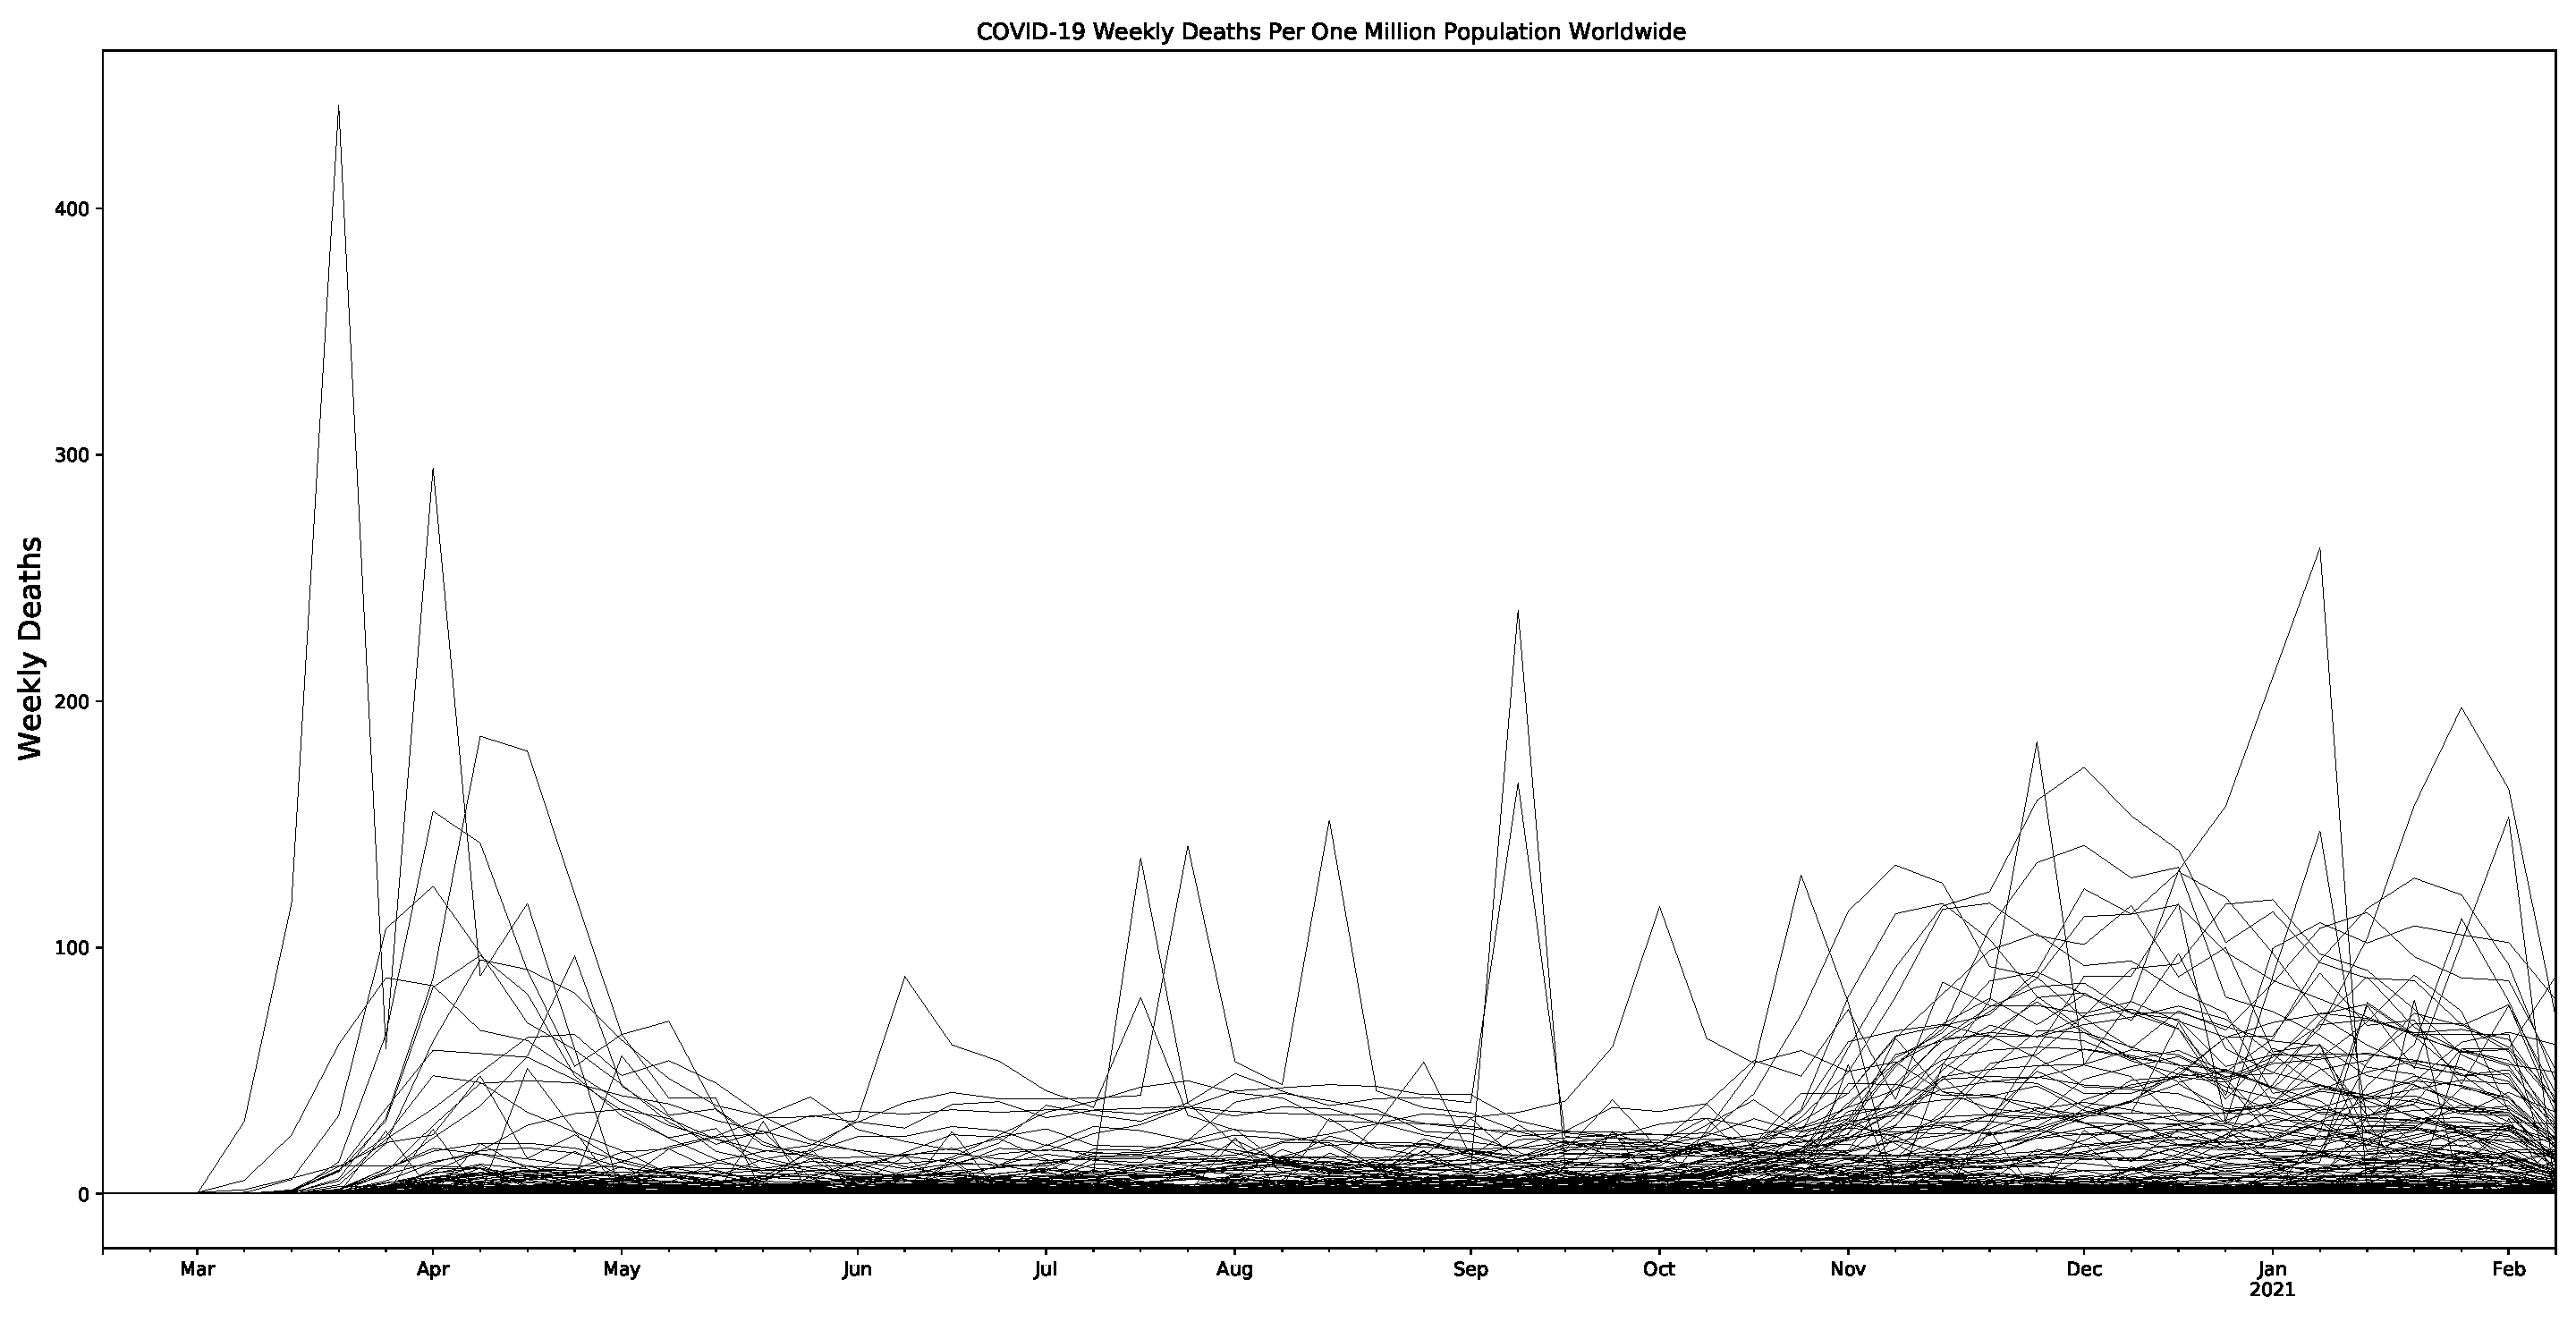
\includegraphics[scale=0.32]{img/weekly-deaths-worldwide.pdf}
    \end{center}
    \vspace{-0.3cm}
    \caption{COVID-19 Weekly Deaths Per One Million Population Worldwide}
\end{figure}
\noindent
To clean the mess, find patterns and extract the required knowledge, a
clustering algorithm was used. This unsupervised learning technique groups
similar data curves together.
\subsubsection{Clustering time series data}
When taking into account time series clustering algorithm, there have been
several measures applied. For example there is probability-based distance, that
takes into account the seasonality of data, Hausdorff distance defined as "the
maximum of the distances from a point in any of the sets to the nearest point in
the other set" (Rote (1991)) or Hidden Markov model based distance used in
modelling complex time series (Zeng, Duan, and Wu (2010)). The most popular
however is the Euclidean distance and Dynamic Time Warping distance. It has been
proven that the Euclidean distance is the most efficient, but forces both time
series to be the same length. The DTW method is however known to be the most
accurate.\\
\\
\textbf{Euclidean vs. Dynamic Time Warping}\\
The main difference between both distances can be best understood graphically.
The picture below shows an example of matched points of two data vectors. They
were connected based on the minimal distance between points based on DTW (black)
and Euclidean (red) distance. It can be seen that with DTW the 11th blue point
matches 4 green points. When taking into account the Euclidean distance it can
be seen that the assigned points 9-to-9 and 10-to-10 are visibly further than
9-to-11 and 10-to-11. That can significantly impact the overall distance of
series between each other. The DTW takes into account the shape of both time
series much better. Dynamic Time warping is a method of calculating distance
that is more accurate than Euclidean distance. It has an advantage over
Euclidean if data points are shifted between each other and we want to look
rather at its shape.
\begin{figure}[H]
    \begin{center}
        \hspace*{-0.3cm}
        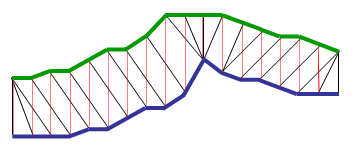
\includegraphics[scale=1.1]{img/euclidean-dtw.png}
    \end{center}
    \vspace{-0.2cm}
    \caption{Visual comparison of matched points based on DTW (black) and Euclidean (red) distance}
\end{figure}
\noindent
Additionally, the two time series don't have to be equal in length as required
by the Euclidean distance. The Euclidean distance takes pairs of data points and
compares them to each other. DTW calculates the smallest distance between all
points --- this enables a one-to-many match.\\
\\
Two K-means clustering models were built: one using the euclidean distance and
one using the DTW algorithm. To this end, \texttt{tslearn}, a Python package
that provides machine learning tools for the analysis of time series, was used.
This package builds on (and hence depends on) the \texttt{scikit-learn},
\texttt{numpy} and \texttt{scipy} libraries.\\
\\
First of all, the optimal number of clusters was evaluated using the mean
silhouette coefficient for all samples. The different silhouette values obtained
for the K-Means Model are listed below:
\begin{itemize}
    \item 2 Clusters silhouette:
    \begin{itemize}
        \item Euclidean distance: $0.63$ --- Dynamic Time Warping: $0.71$
    \end{itemize}
    \item 3 Clusters silhouette:
    \begin{itemize}
        \item Euclidean distance: $0.56$ --- Dynamic Time Warping: $0.66$
    \end{itemize}
    \item 4 Clusters silhouette:
    \begin{itemize}
        \item Euclidean distance: $0.58$ --- Dynamic Time Warping: $0.66$
    \end{itemize}
    \item 5 Clusters silhouette:
    \begin{itemize}
        \item Euclidean distance: $0.59$ --- Dynamic Time Warping: $0.63$
    \end{itemize}
\end{itemize}
The best value for the mean silhouette coefficient is obtained with only $2$
clusters. However, taking into account our knowledge of the phenomenon, we
expect to find $3$ clusters of countries: those hardly hit by both the first and
the second wave, those that have been hit by either the first or the second
wave, and those suffering COVID-19 deaths constantly. Two K-means models with
3 clusters were therefore evaluated: one trained using the euclidean distance
and the other using the dynamic time warping algorithm.
\begin{figure}[H]
    \begin{center}
        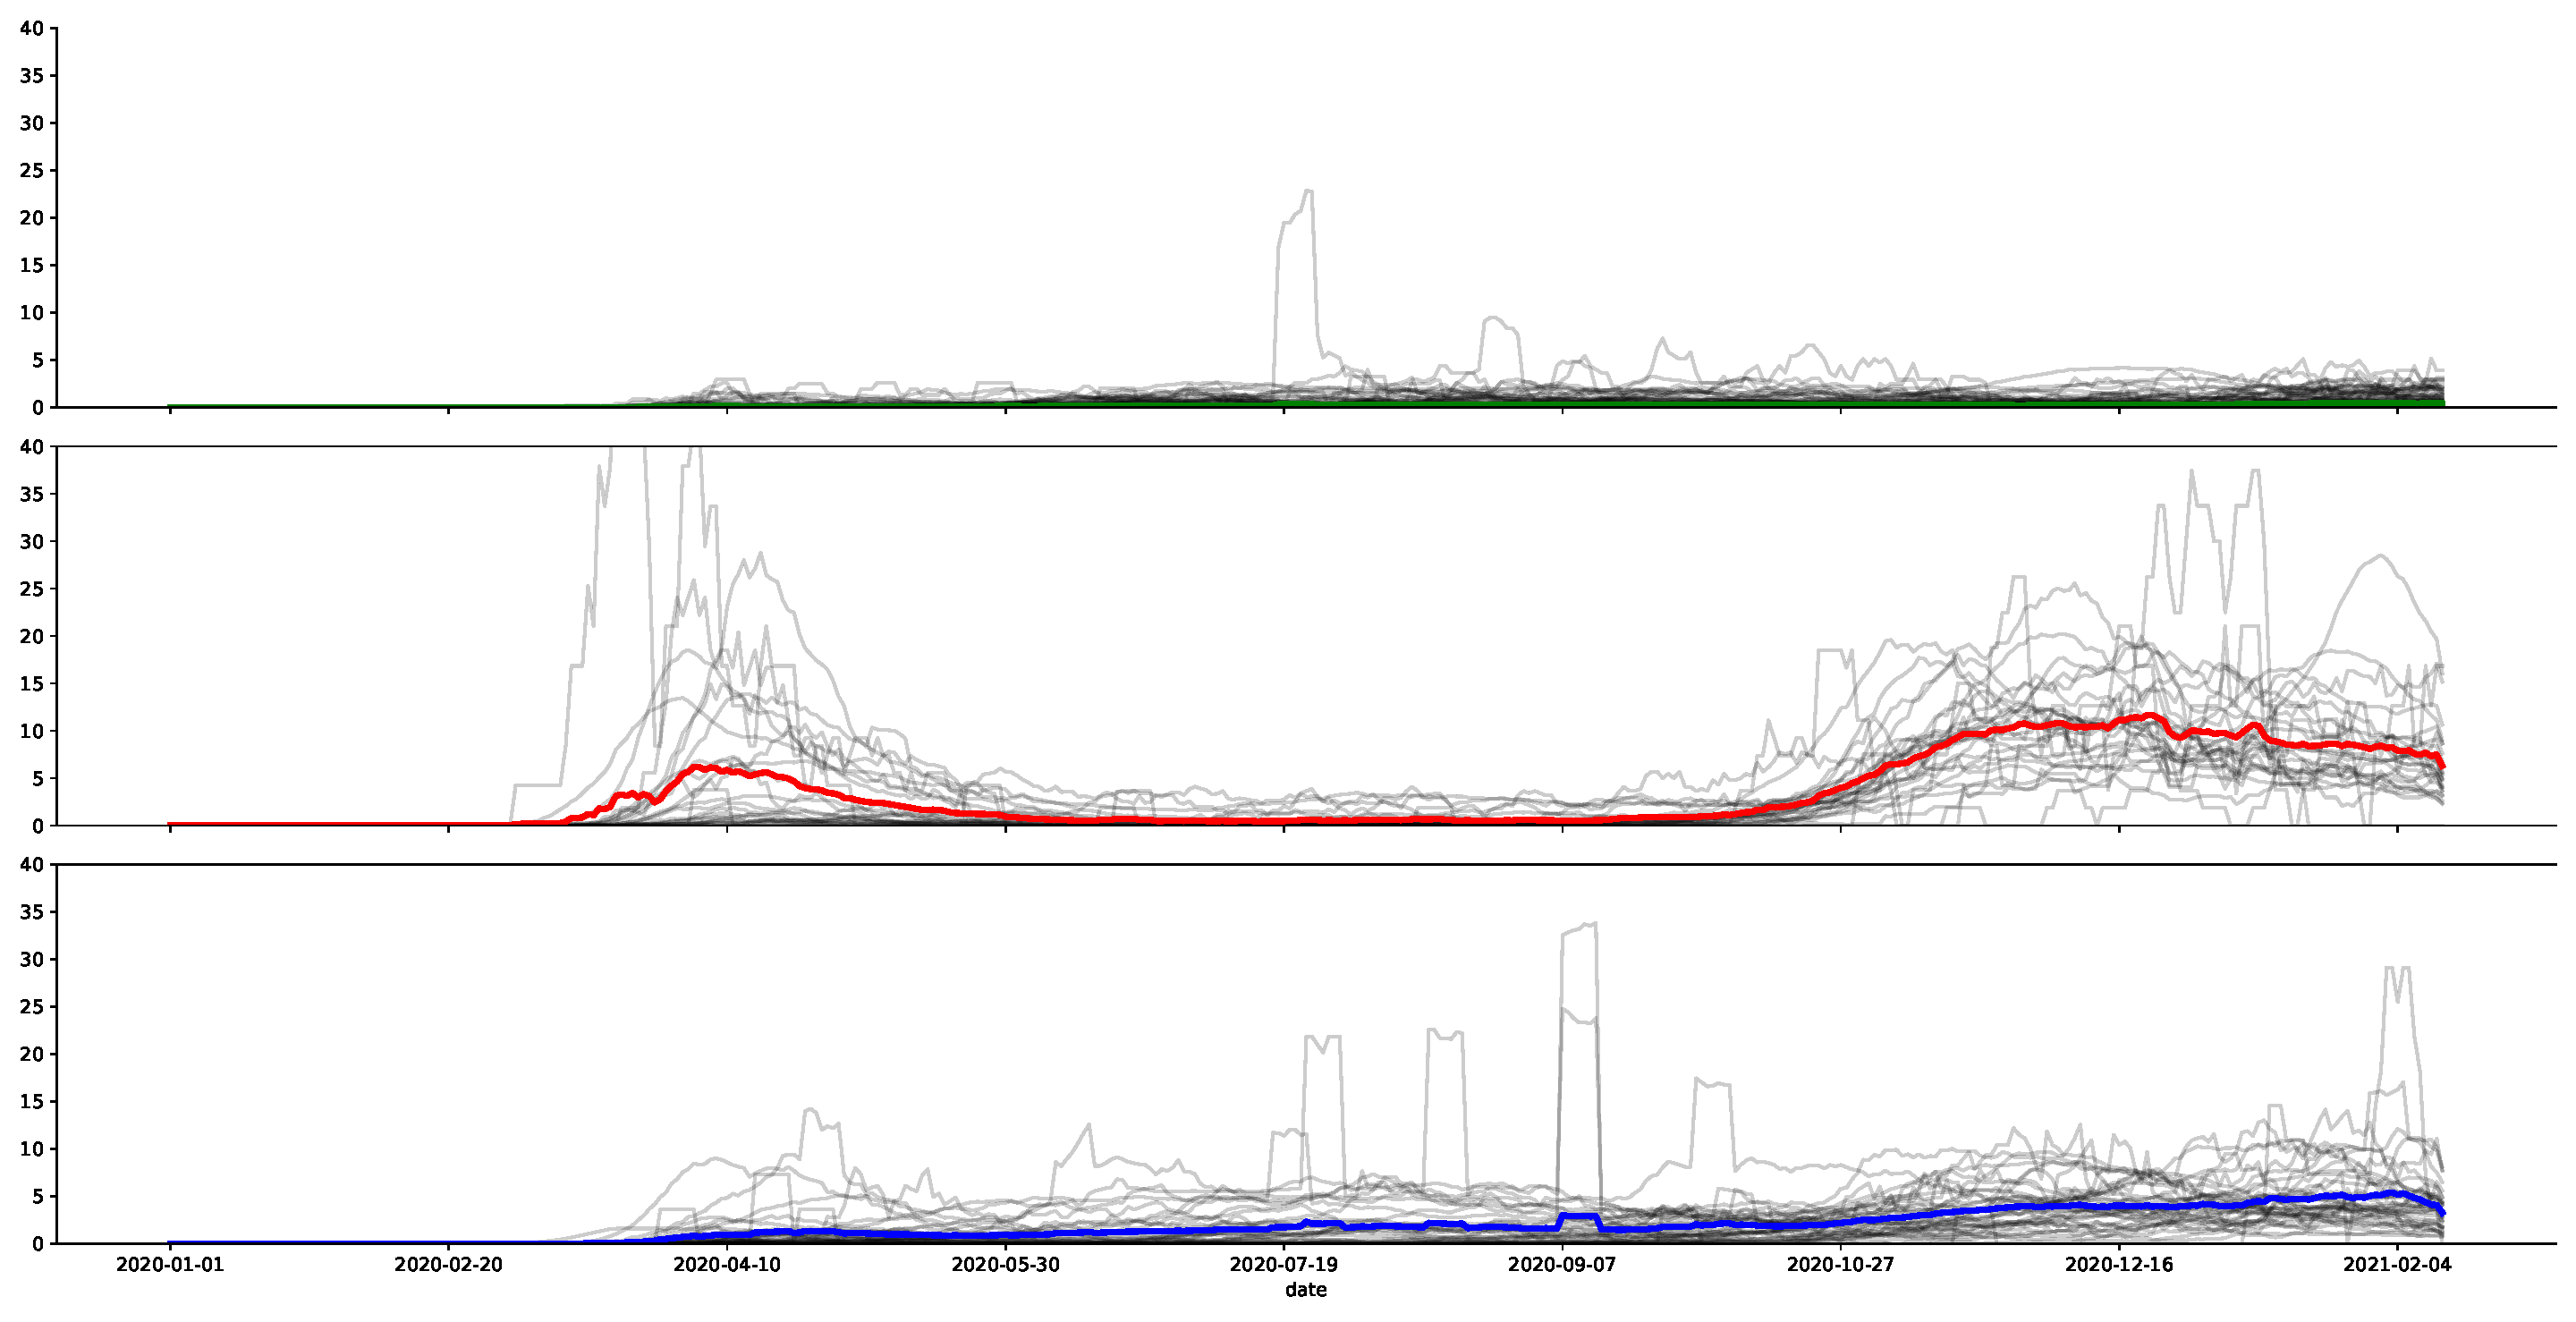
\includegraphics[scale=0.32]{img/daily-deaths-euclidean-clusters.pdf}
    \end{center}
    \vspace{-0.3cm}
    \caption{Time series K-means Clustering Model using Euclidean distance}
\end{figure}
\noindent
Figure 6 shows the clusters obtained by applying the K-means Clustering
algorithm provided by the \texttt{TimeSeriesKMeans} class of the
\texttt{tslearn} Python package. In this model, the metric chosen to be used for
both cluster assignment and barycenter computation is the euclidean distance:
\begin{itemize}
    \item the {\color{ForestGreen}green cluster} groups $147$ countries with
    daily deaths close to zero;
    \item the {\color{blue}blue cluster} groups $39$ countries which suffer
    constantly COVID-19 deaths and where it seems the situation is getting worse
    and worse over time;
    \item the {\color{red}red cluster} groups $19$ countries with a huge number
    of daily deaths, that managed to get the situation controlled for a while,
    but are now suffering for the second wave;
    \item mean silhouette coefficient for all samples: $0.60$.
\end{itemize}
The time series K-means clustering model using the Dynamic Time Warping
algorithm provides different clusters. As shown in figure 7,
\begin{itemize}
    \item the {\color{ForestGreen}green cluster} groups $139$ countries;
    \item the {\color{blue}blue cluster} groups $44$ countries;
    \item the {\color{red}red cluster} groups $22$ countries;
    \item mean silhouette coefficient for all samples: $0.66$.
\end{itemize}
We should keep in mind that the DTW algorithm is quite CPU-intensive: as a
matter of fact, with $50$ iterations, the same number used to obtain the model
with the euclidean distance, it takes almost $2$ minutes\footnote{Please take
this statistic as a very general one --- it is relative to an Intel Core
i7-7700K Processor (4 Cores 8 Threads @ 4.20 GHz).} to compute the clusters
shown in figure 7.
\begin{figure}[H]
    \begin{center}
        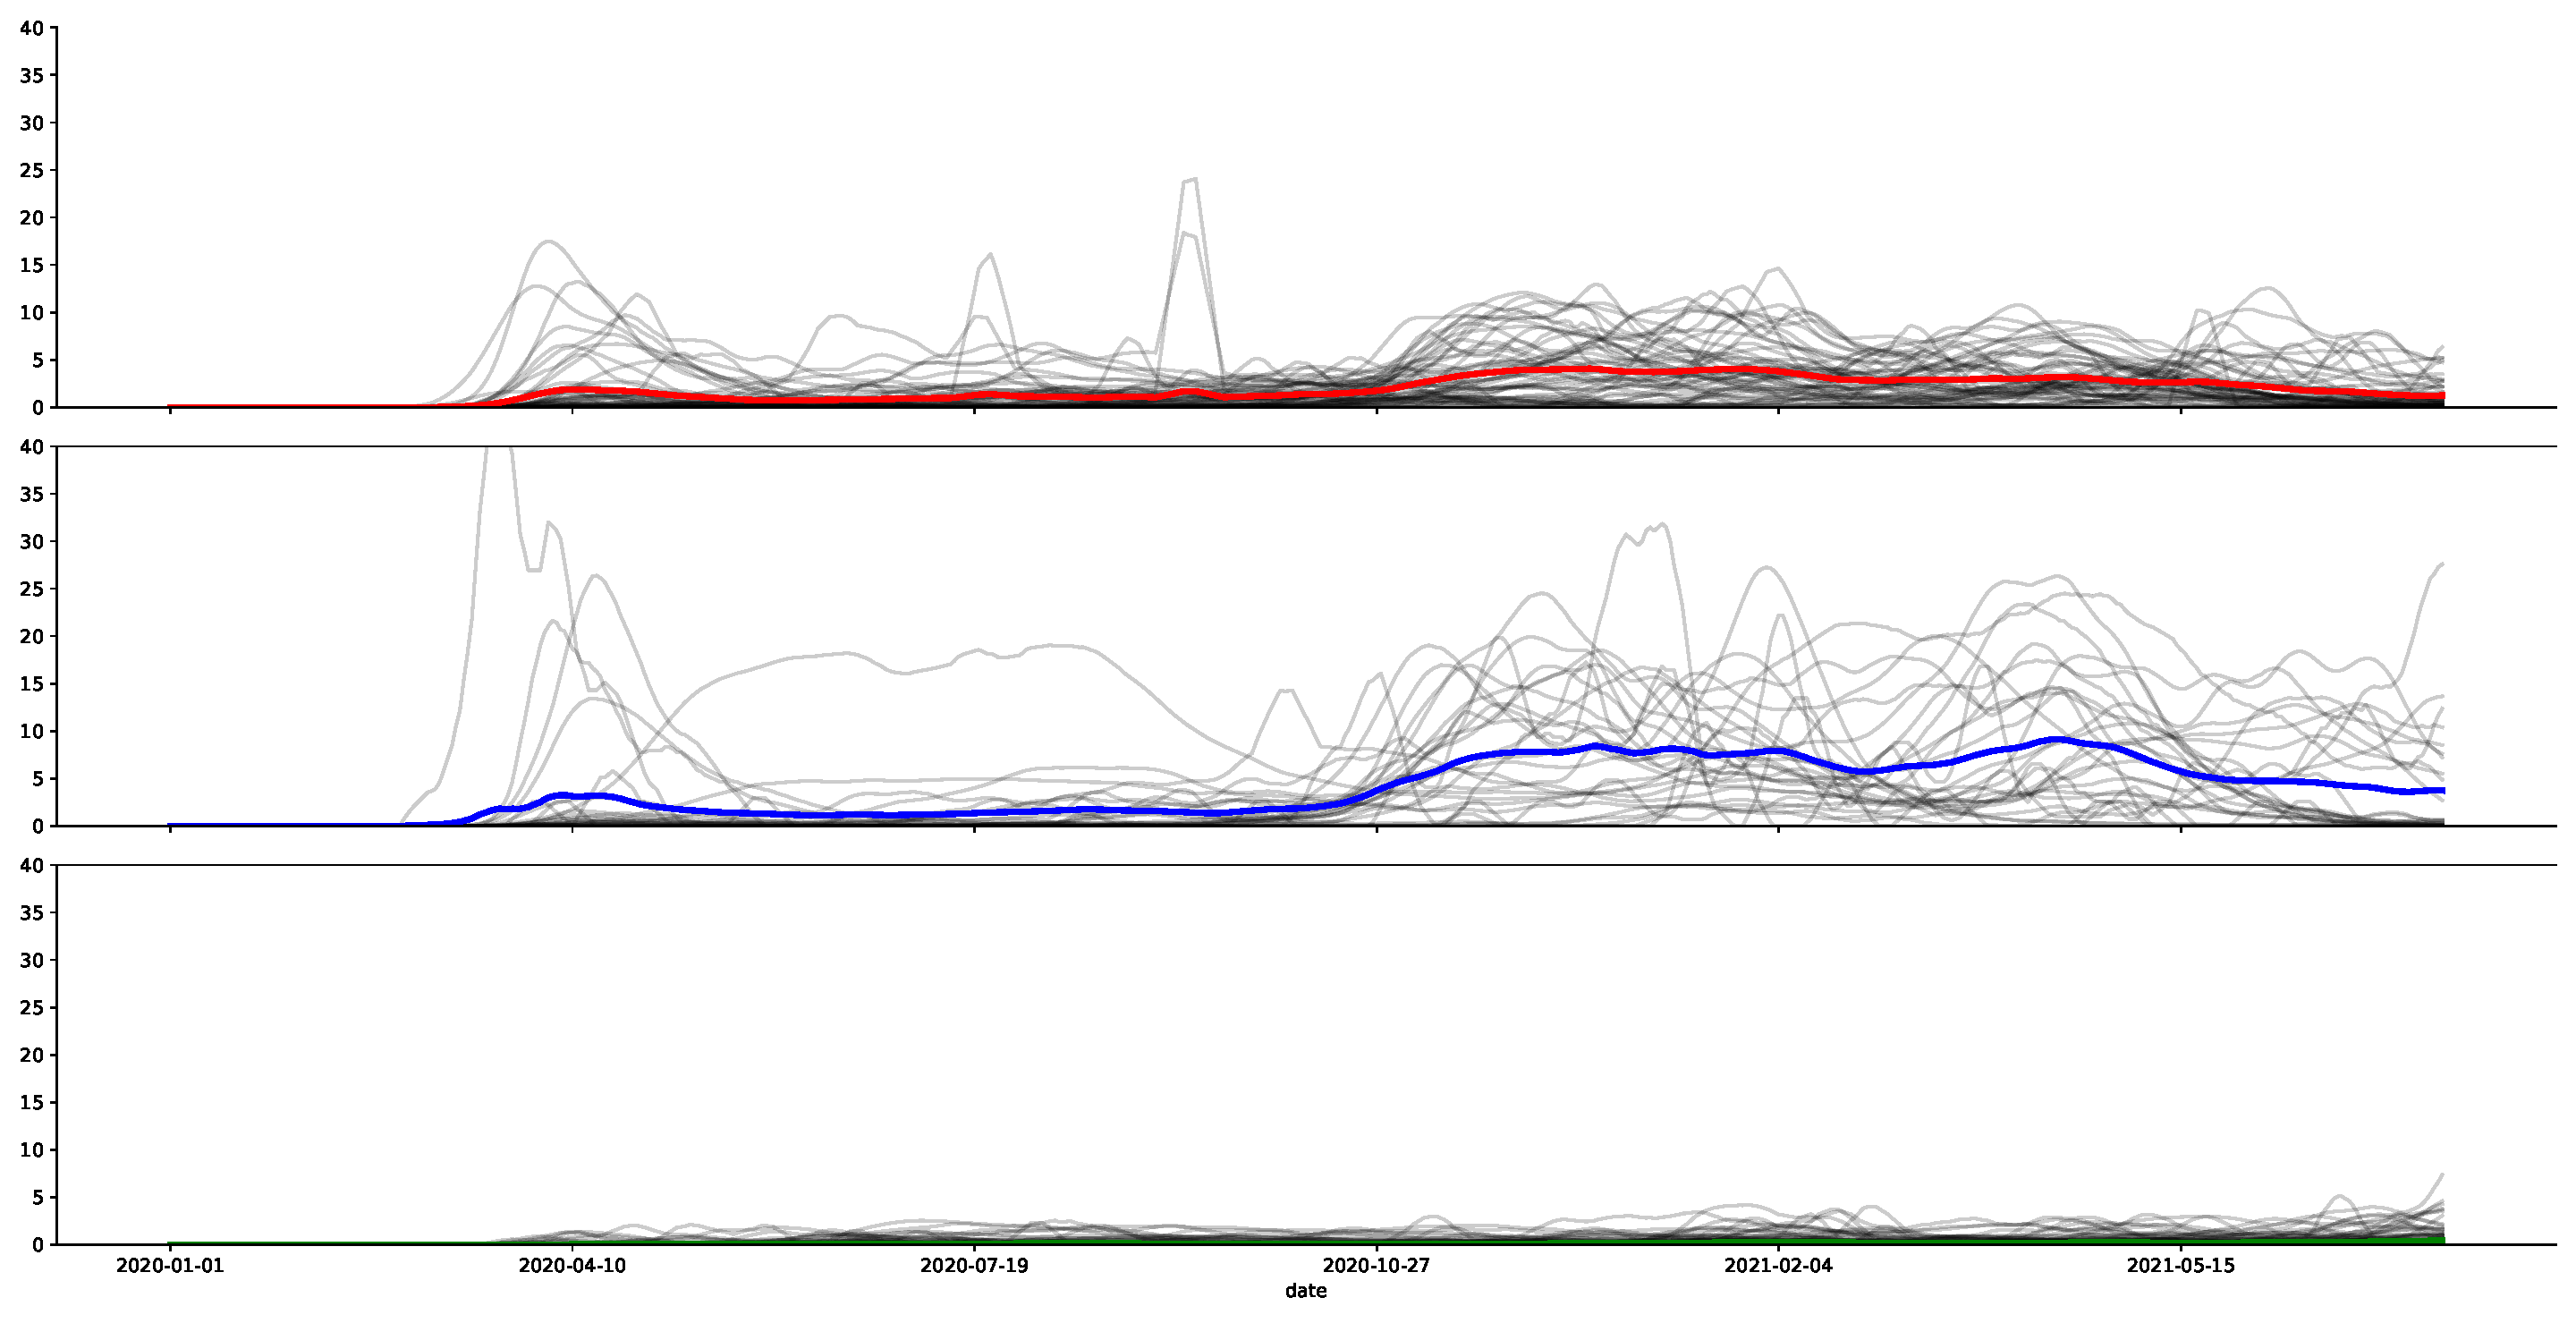
\includegraphics[scale=0.32]{img/daily-deaths-dtw-clusters.pdf}
    \end{center}
    \vspace{-0.3cm}
    \caption{Time series K-means Clustering Model using Dynamic Time Warping algorithm}
\end{figure}
\noindent
To compare the two models, as there is no ground truth when dealing with
clustering problems, I represented the clusters obtained by the two models on
the world map. Surprisingly enough, as shown in figure 8 and in figure 9,
those groups form local clusters on the world map as well. The nature of the
phenomenon we are analysing, the spread of the SARS-CoV-2 pandemic, tells us
that how well this local clusters are grouped in the world map, in terms of
neighboring countries can be used as a measure of how well the algorithm
performed:
\begin{figure}[H]
    \begin{center}
        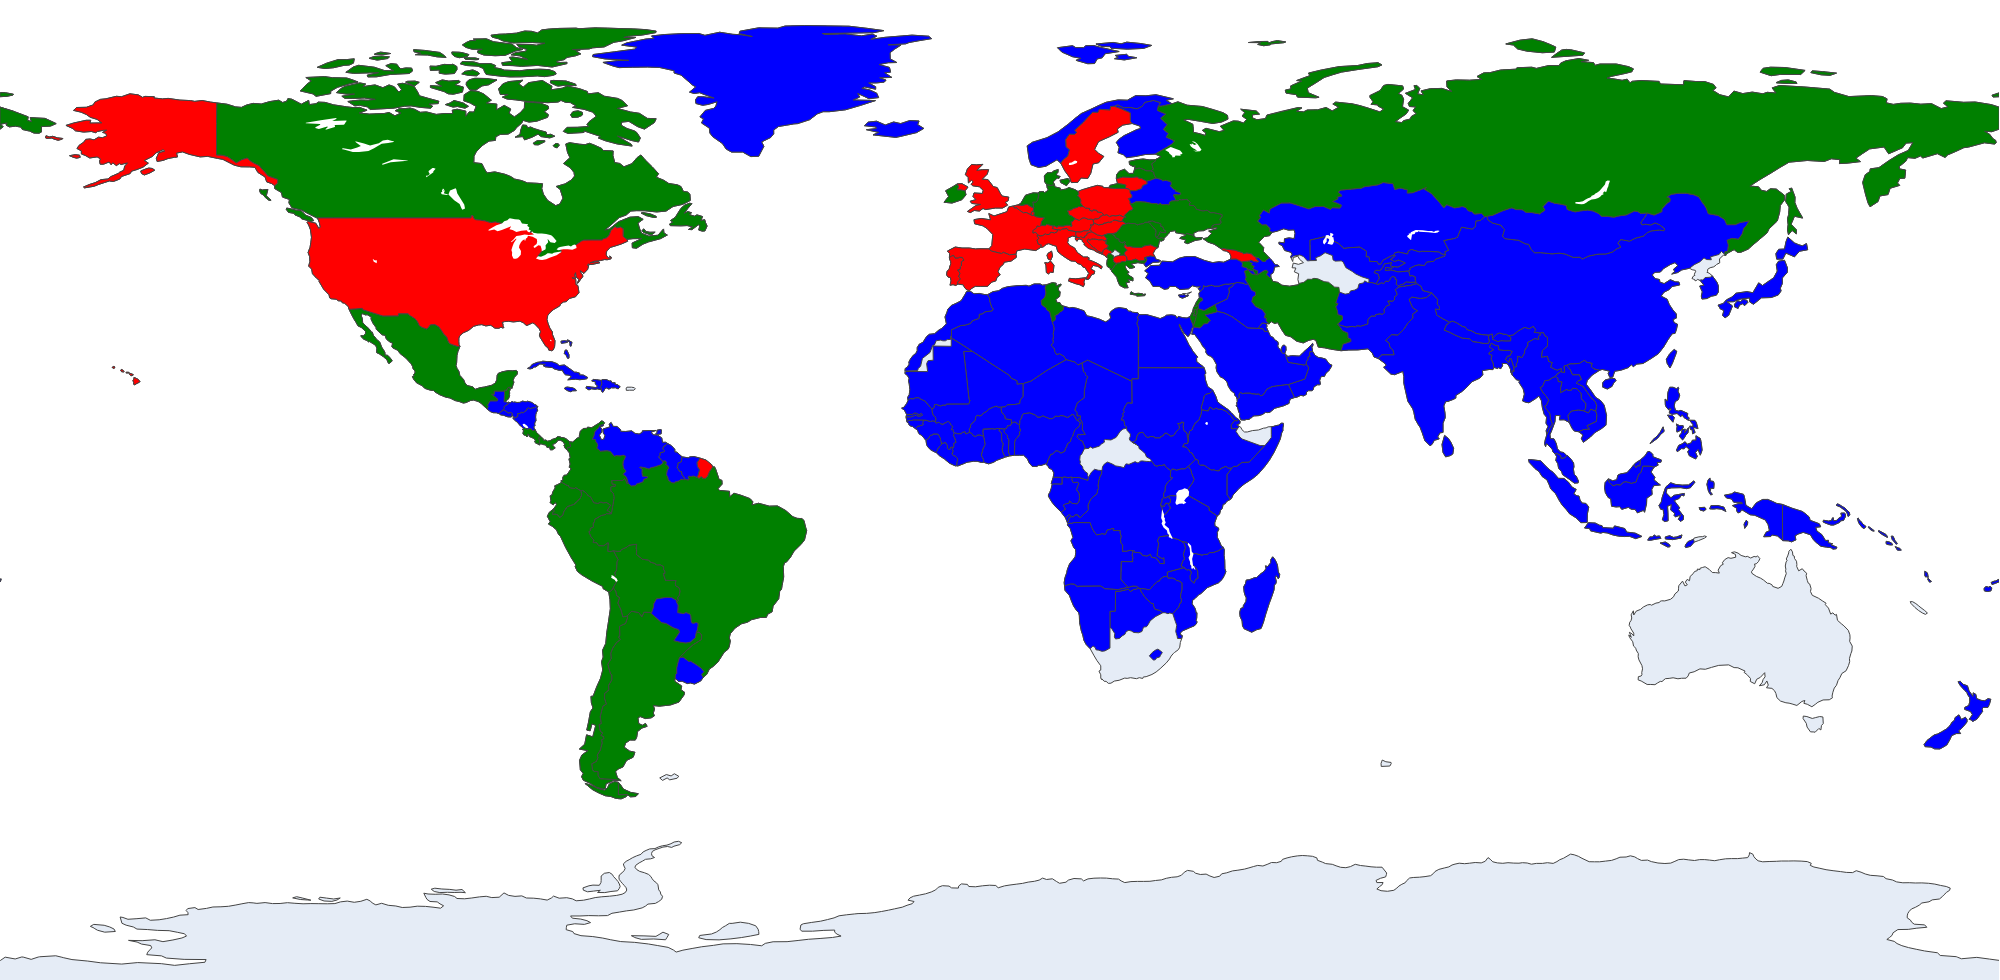
\includegraphics[scale=0.22]{img/euclidean-clusters-map.png}
    \end{center}
    \vspace{-0.2cm}
    \caption{K-means Clustering Model Worldwide Map (Euclidean Distance)}
\end{figure}
\noindent
A quick look at the map below shows that the red cluster is located on the
European continent. Furthermore, countries from the blue cluster are
concentrated in Russia, the middle east and African continent.
\begin{figure}[H]
    \begin{center}
        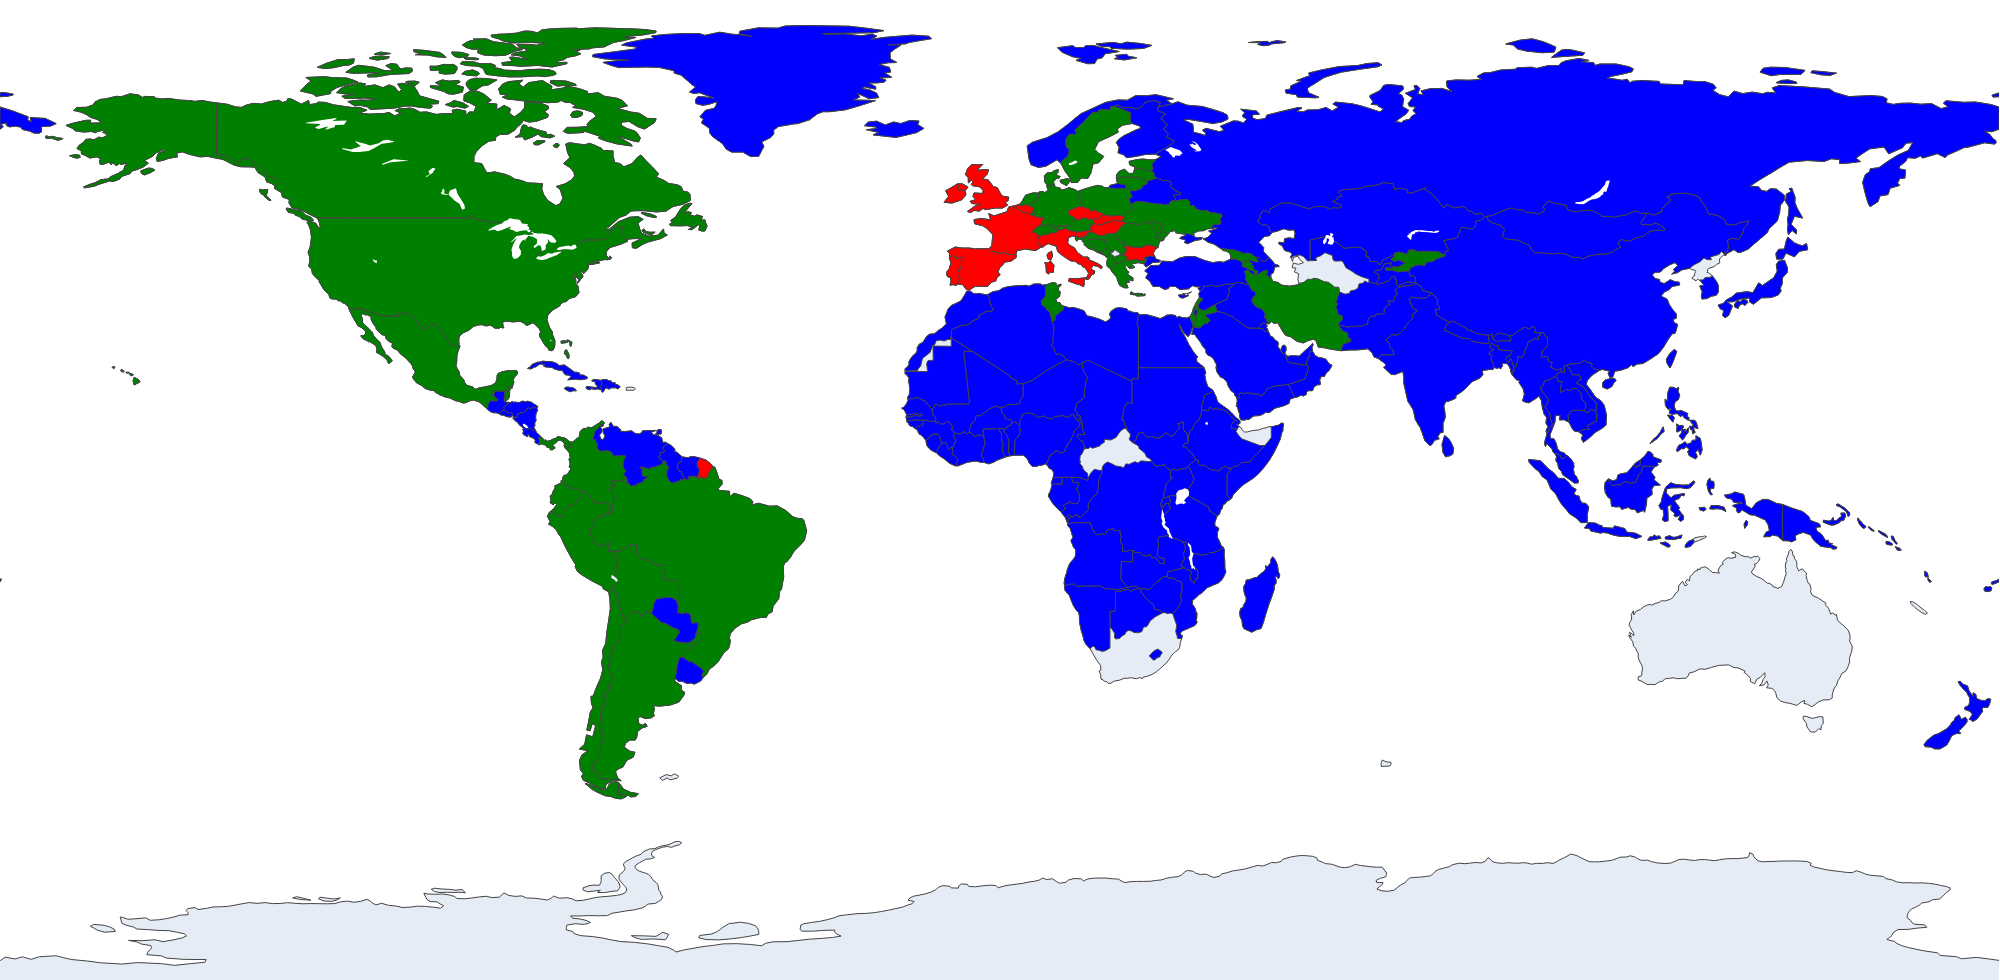
\includegraphics[scale=0.22]{img/dtw-clusters-map.png}
    \end{center}
    \vspace{-0.2cm}
    \caption{K-means Clustering Model Worldwide Map (DTW Algorithm)}
\end{figure}
\noindent
One important observation to be made is that changing from the euclidean
distance to the DTW algorithm, the US moves from the {\color{red}red cluster} to
the {\color{ForestGreen}green cluster}. Also, the Russian Federation moves from
the {\color{ForestGreen}green cluster} to the {\color{blue}blue cluster}. This
is understandable if we take into account that the US has a population of
$328.2$ million while the Russian Federation has a population of $144.4$
million.\\
\\
Just by observing the two world maps presented, it goes without saying that the
DTW Model performed better.
\subsection{Personalized predictive models for symptomatic COVID-19 patients}

%-------------------------------------------------------------------------------
% Section: Conclusion
%-------------------------------------------------------------------------------
\newpage
\section{Conclusion}

%-------------------------------------------------------------------------------
% Section: Software Architecture
%-------------------------------------------------------------------------------
\newpage
\section{Software Architecture}

%-------------------------------------------------------------------------------
% Bibliography
%-------------------------------------------------------------------------------
\newpage
\printbibliography

\end{document}
